\documentclass[unknownkeysallowed]{beamer}

\mode<presentation>
{
   \usetheme[secheader]{Boadilla}
 % \usetheme{Warsaw}
  % or ...

  %\setbeamercovered{transparent}
  % or whatever (possibly just delete it)
}


\usepackage[english]{babel}
% or whatever

\usepackage[utf8]{inputenc}
% or whatever

\usepackage{xmpmulti}
\usepackage{times}
\usepackage[T1]{fontenc}
% Or whatever. Note that the encoding and the font should match. If T1
% does not look nice, try deleting the line with the fontenc.

\usepackage{pifont}% http://ctan.org/pkg/pifont
\newcommand{\cmark}{\ding{51}}
\newcommand{\xmark}{\ding{55}}%

\usepackage{tikz} 
\tikzstyle{every picture}+=[remember picture]
\usetikzlibrary{arrows,shapes,trees}

\def\no{\hbox{\bf not} \; }
\def\noo{\hbox{\bf not}}
\def\oor{{\:\hbox{\it or}\: }}
\def\mnot{{- \hbox{\bf not}}}
\def\naf{\: \hbox{\em not} \:}
\def\la{{\leftarrow
}}


%\renewcommand{\labelitemi}{$\circ$}
%\renewcommand{\labelitemii}{$\triangleright$}


\title[Beliefs and Truthfulness of Agents] % (optional, use only with long paper titles)
{\large An Answer Set Programming Framework for \\
Reasoning about Agents' Beliefs and Truthfulness of Statements}

%\subtitle
%{Theory and Applications} % (optional)

\author[Balduccini, Gelfond, Pontelli, Son]
{ 
Marcello Balduccini
\includegraphics[width=0.1in]{sju.jpg}, 
Michael Gelfond
\includegraphics[width=0.1in]{ttu.jpg}, and \\ 
Enrico Pontelli and Tran Cao Son
\includegraphics[width=0.1in]{nmsu.png}
} % Author(s)

\institute[ ]
{

\includegraphics[width=0.2in]{nmsu.png}~Computer Science Department, New Mexico State University, Las Cruces, NM \\

\includegraphics[width=0.2in]{ttu.jpg}~Computer Science Department, Texas Tech University, Lubbock, TX \\

\includegraphics[width=0.2in]{sju.jpg}~Department of Decision \& System Sciences, Saint Joseph's University, Philadelphia, PA 
} % Institution(s)
 
 
\date[KRR-2020] % (optional)
{KRR 2020}

\subject{Talks}
 
% \pgfdeclareimage[height=0.5cm]{university-logo}{university-logo-filename}
% \logo{\pgfuseimage{university-logo}}

 
% Delete this, if you do not want the table of contents to pop up at
% the beginning of each subsection:
\AtBeginSection[]
{
  \begin{frame}<beamer>{Outline}
    \tableofcontents[currentsection,currentsubsection]
  \end{frame}
}


% If you wish to uncover everything in a step-wise fashion, uncomment
% the following command: 

%\beamerdefaultoverlayspecification{<+->}


\begin{document}

\maketitle

\section{Motivation and Contributions} 



\begin{frame}{Example} 

{\small
\begin{center} 
\begin{tabular}{c|p{0.7\textwidth}}
\hline\hline
Time step & Information \\
\hline 
\textbf{$0$} &  John says that his family is poor (\alert{$poor$}). \\
\textbf{$1$} &  We observe  that John attends an expensive college (\alert{$expensive\_college$}). \\
\textbf{$2$} &  We learn that John has a full scholarship  because of his financial hardship (\alert{$has\_scholarship$}). \\
%\textbf{$3$} &  We learn that John buys an expensive house  (\alert{$buy\_expensive\_house$}). \\
\hline\hline
\end{tabular} 
\end{center} 
Is John's statement about his family's financial status truthful? 

\begin{itemize}  
\vspace{-2pt}
\item at time 0? \alert{Yes} (\textcolor{blue}{there is nothing that proves otherwise.})

\vspace{-2pt}
\item at time 1? \alert{No} (\textcolor{blue}{by default, attending expensive college requires lots of money.}) 
[\alert{$d_1$}] 

\vspace{-2pt}
\item at time 2? \alert{Yes} (\textcolor{blue}{by default, financial hardship scholarship is only for low income families.})
[\alert{$d_2$} and $d_2$ is \emph{\bf more preferred than} $d_1$] 

%\vspace{-2pt}
%\item at time 3? \alert{No} (\textcolor{blue}{by default, a student does not have money to afford an expensive house.})

%\item Is John's statement about his family's financial situation truthful at time 0? (\alert{Yes}); 
%
%\item Is John's statement about his family's financial situation truthful at time 1? \alert{No} 
%
%\item Is John's statement about his family's financial situation truthful at time 2? \alert{Yes} 

%\item \textbf{Time step $0$}: John says that his family is poor (\alert{$poor$}). 

%It is likely that we would believe John---since we have nothing to conclude otherwise. 

%\item \textbf{Time step $1$}:  We observe the fact that John attends an expensive college ($in\_college$). 

%%\emph{Since students attending the college are normally from rich families} (default $d_1$), this might lead us to  conclude that John has lied to us. We indicate that  the default $d_1$ is the reason to draw such conclusion. 
%
%\item \textbf{Time step $2$}: We learn the fact that John has a complete scholarship  because of his financial hardship ($has\_scholarship$). 
%
%\emph{Since a student's hardship is usually derived from the family's financial situation} (default $d_2$), this fact would  allow us to withdraw the conclusion that John is a liar made at  time instance $t_1$. It is still insufficient for us to conclude that  John's family is poor. 
%
%The situation might be different if, for example, we have a preference among defaults. In this example, if we are inclined to believe in the conclusion of $d_2$ more than that of $d_1$, then we would believe that John's family is poor and thus restore our trust in John's statement. 
% 
\end{itemize} 
}

%\begin{itemize}  
%\item Represent the knowledge base and default rules of the agent as a logic program $\Pi_K$  
%\item Represent actions and their effects as a logic program $\Pi_A$ 
%\item Encode observations as facts $\Pi_O$ 
%\item Develop method for evaluation of statements of agents. 
%\end{itemize}  
\end{frame} 

\subsection*{Research Problem}
\begin{frame}{}

In everyday life,  agents observe  the world, receive information from others, 
and make  judgment about the truthfulness of information provided by others. 
\alert{
How do they reach their conclusion? 
}

\begin{center}
\only<1>{
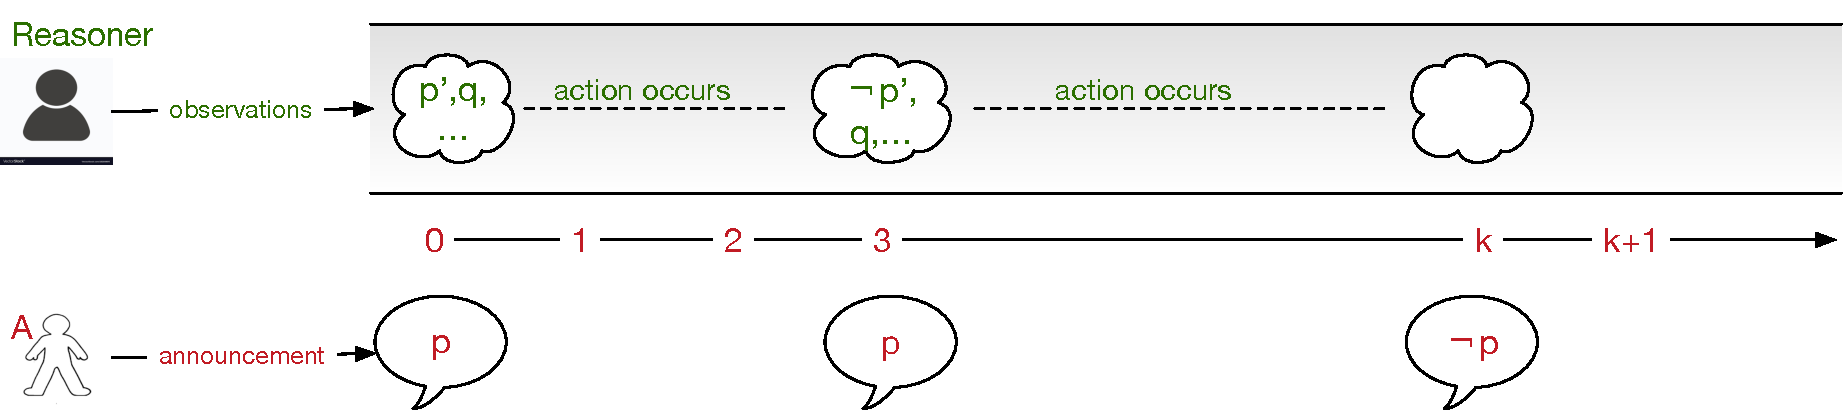
\includegraphics[width=0.95\linewidth]{timeline.pdf}} 

\only<2>{
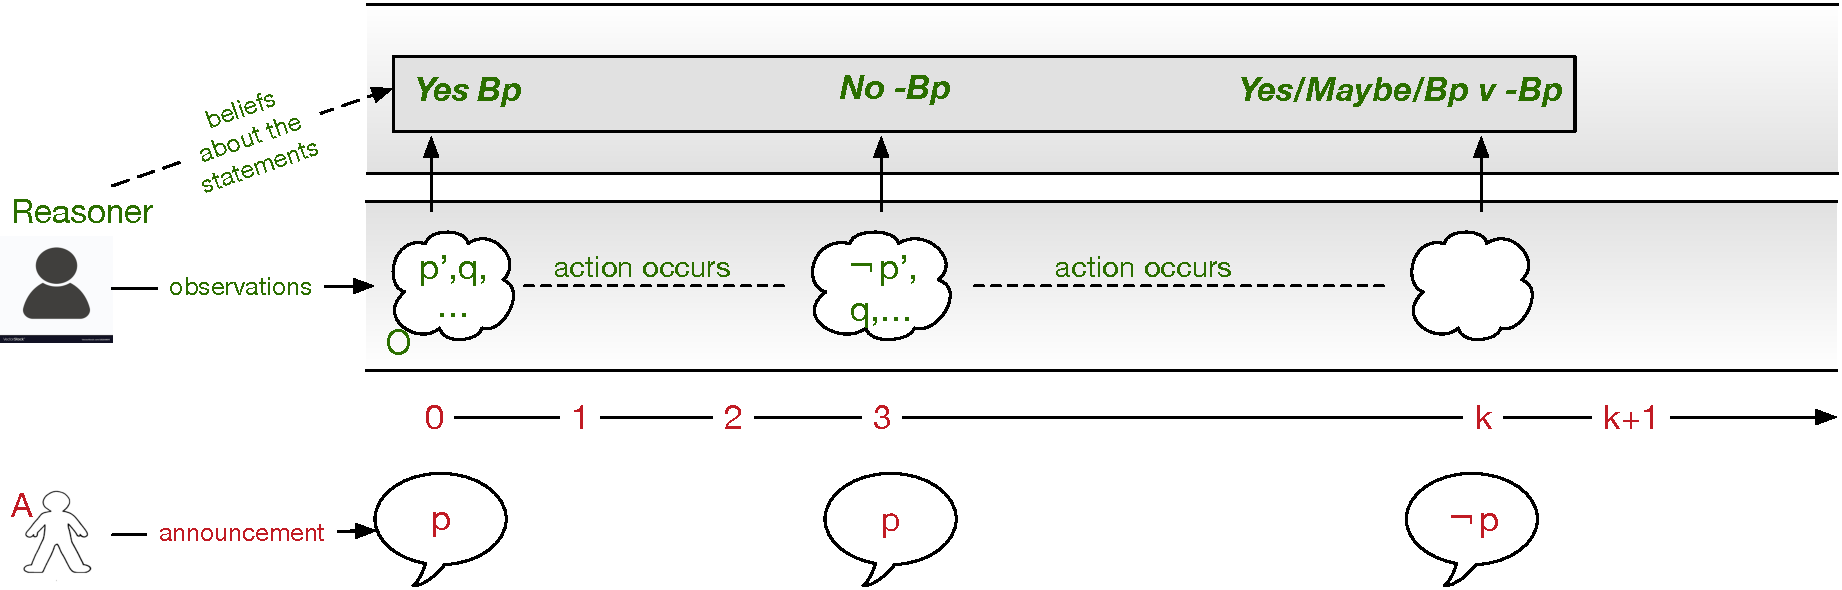
\includegraphics[width=0.95\linewidth]{timeline-with-judgement.pdf}
}
\end{center}

\only<1>{
\alert{Questions:} (by the reasoner) does A tell the truth? 
}



\only<2>{
{\small 
\alert{Questions:} 
\begin{enumerate} 
\item Can the statement about property $p$ made by agent $A$ believed to be true?       
\item Which statements of other agents does the reasoner believe to be true? false?  
\end{enumerate} 
}
}
 
\end{frame} 




\begin{frame}{Contributions}


\begin{enumerate}
\item An abstract model for representing and reasoning about 
\begin{enumerate}
\item the evolution of an agent's beliefs over time; and 
\item truthfulness of third-party statements;   
\end{enumerate}
\item A concrete realization of the model using
Answer Set Programming; and
\item A demonstration of the proposed framework on an important problem in the
        area of  cyber security. 
\end{enumerate}

%
%Develop  a system for reasoning about truthfulness of statements made by other agents given 
%\begin{itemize} 
%\item statements made by agents;  
%\item observations made along a history, i.e., facts at different time points about  
%\begin{itemize} 
%\item   properties of the world; and  
%\item actions executed by other agents; 
%\end{itemize}
%\item an action theory that encodes knowledge about actions, their effects and pre-conditions; and 
%\item a default theory that encodes the preferences (or biases) of the reasoner for commonsense reasoning and dealing with incomplete information. 
%\end{itemize} 
 
\end{frame} 
 
\section{Beliefs about and Truthfulness of Statements}

\subsection*{General Framework}

\begin{frame}{}  


\begin{block}{Assumptions (about the reasoner)} 
\begin{itemize}  
\vspace{-2pt}
\item \alert{optimistic in nature}: an agent believes a statement made by   another agent unless  there is a reason to believe otherwise!   
\vspace{-2pt}
\item \alert{commonsense reasoner}:  an agent uses default reasoning to draw  conclusions about truthfulness of statements made by other agents. 
\vspace{-2pt}
\item \alert{observant}:  an agent observes other agents and will use her observations in draw conclusions.
\vspace{-2pt}
\item \alert{active}:  an agent executes her own actions to change the world.
\end{itemize}  
\end{block} 

\end{frame} 
  

\begin{frame}{} 

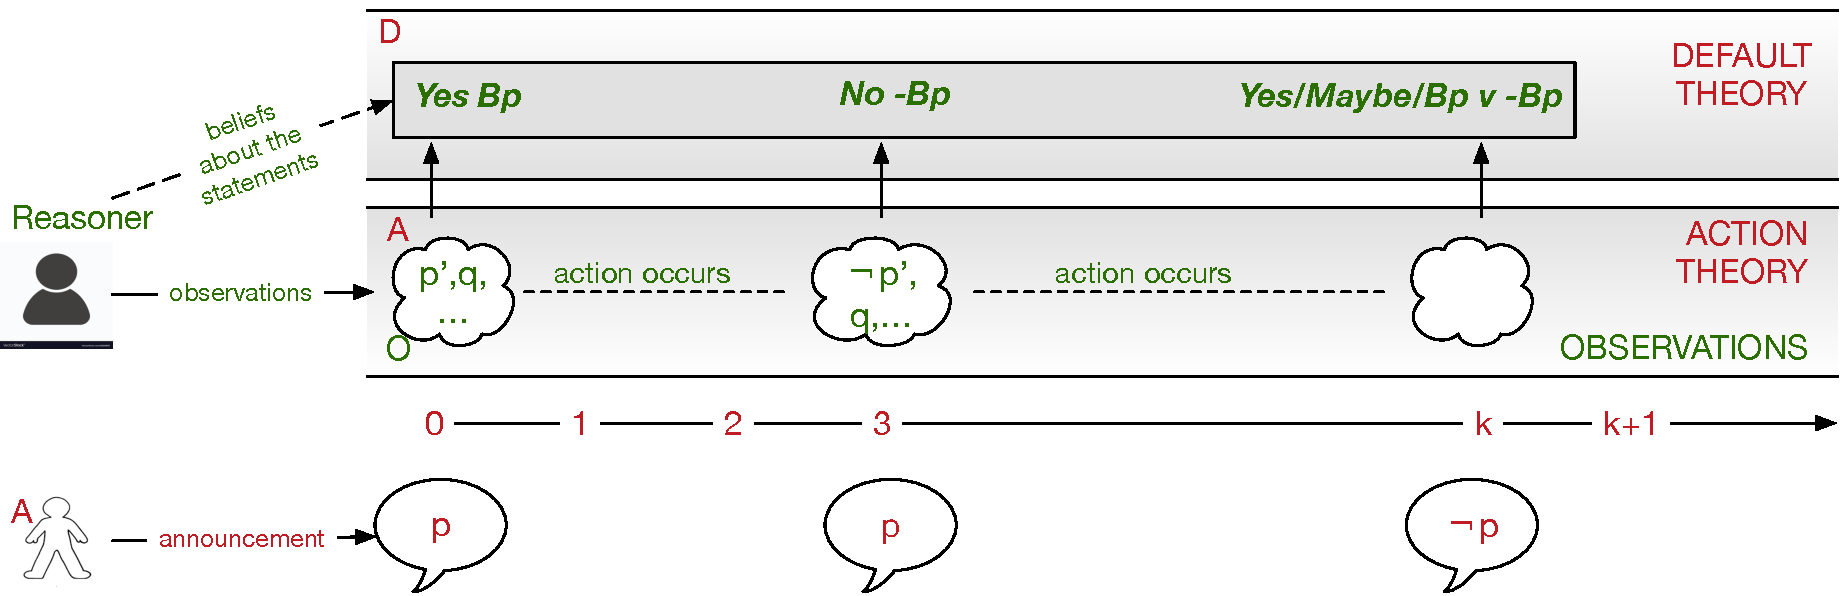
\includegraphics[width=0.95\linewidth]{framework.pdf}
 

\begin{block}{Solution} 
\begin{itemize}  
\vspace{-2pt}
\item Represent the knowledge base and default rules of the agent by a default theory  $\mathit{Def}$. 
\vspace{-2pt}
\item Represent actions and their effects by an action theory  $A$.
\vspace{-2pt}
\item Represent observations by a set of facts $O$. 
\vspace{-2pt}
\item Separate beliefs of the reasoner and the properties of the world. 
\vspace{-2pt}
\item Develop method for evaluation of statements of agents (define $\mathit{Def} \cup A \cup O \models p[t]$ for $p$ is believed to be true at time $t$ ). 
\end{itemize}  
\end{block} 
 
\end{frame} 
  
\subsection*{Entailment}

\begin{frame}{ }

% 
%  
%\begin{itemize}
%%
%\item \alert{Observations}: action occurrences $O_a$ and fluent values  
%$O_w$;  
%%
%\item \alert{Action theory}:  $Act$ in a suitable logic $A$ that defines $\models_A$ 
%\[
%Act \cup O_a \cup I \models_A p \: \: \mathbf{ after } \: \: [a_0,\ldots,a_n] 
%\] 
%$p$ is true after the execution of   $[a_0,\ldots,a_n]$ 
%from the state $I$.
%
%\item \alert{Default theory}: $\textit{Def}$ defines $\models_D$,   
%$
%\textit{Def} \cup O \models b
%$ 
%
%$b$ is true w.r.t. the set of observations $O$ and the theory $\textit{Def}$.
% %
%\end{itemize}


 
\begin{itemize} 
\item \alert{Given}: $T = (O_a, O_f, Act, \textit{Def})$ and  $\models_A$ and $\models_D$. 

\begin{itemize}
%
\item \alert{Action theory}:  $Act$ in a suitable logic $A$ that defines $\models_A$ 
\[
Act \cup O_a \cup I \models_A p \: \: \mathbf{ after } \: \: [a_0,\ldots,a_n] 
\] 
$p$ is true after the execution of   $[a_0,\ldots,a_n]$ 
from the state $I$.

\item \alert{Default theory}: $\textit{Def}$ defines $\models_D$,   
$
\textit{Def} \cup O \models b
$ 

$b$ is true w.r.t. the set of observations $O$ and the theory $\textit{Def}$.
 %
\end{itemize}





\item \alert{Question}: Is $b$ true ( false) at a certain time step $t$, denoted by $p[t]$, given $T$? 
\end{itemize} 
\[
T \models b[t] \,\,\Leftrightarrow\,\, \langle W[t], Def \rangle \models_D b \label{entail} 
\]
Steps in determining $b[t]$:
\begin{itemize}
\item $W[t]$: model of the world  at the time step $t$ from  $Act$, $O_a$, and $O_f$ (using $\models_A$); and  
\item Determine  whether $b$ is true  given  $\textit{Def}$ and $W[t]$ (using $\models_D$). 
\end{itemize}

\end{frame}


\section{Reasoning about Beliefs and Truthfulness Using ASP} 

\subsection*{Representation}

\begin{frame}{}

Representation of $T = (O_a, O_w, Act, \textit{Def})$ 
\begin{itemize} 

\item \alert{Observations}: 

%\begin{list}{\textcolor{ngreen}{$\Box$}}{\topsep=2pt \parsep=2pt \itemsep=2pt }

\begin{itemize} 
\item $obs(p, s)$: proposition $p$ is observed at time step $s$. 
\item $occ(a, s)$: action $a$ occurred at time step $s$.
\end{itemize}
%\end{list}


\item \alert{Action theory}: high-level action language  
\cite{GelfondL98}. 

\item \alert{Default theory}: default theory with preferences  \cite{GelfondS98}.  
\end{itemize}

\end{frame}

\subsection*{Implementation}

\begin{frame}{}


Encoding of $T$ by $\Pi(T)$, an answer set program with rules for    
\begin{enumerate}
\item reasoning about actions and observations, defining $holds(f, t)$: 

$f$ is true at step $t$; 
 
\item reasoning about defaults, defining $believes(b,t)$: 

$b$ is believed to be true at step $t$. 
\end{enumerate} 

\begin{block}{Entailment between $T$ and $stm(b,s)$, $t \ge s$}
\begin{itemize} 
\item $T \models {+}stm(b,s)@t$  if  $\Pi(T) \models believes(b,t) $; 

\item $T \models {-}stm(b,s)@t$  if $\Pi(T) \models believes(\overline{b},t)$  

\item $T \not\models {\pm}stm(b,s)@t$     
if $T \not\models +stm(b,s)@t$ and $T \not\models -stm(b,s)@t$.

\end{itemize}  
\end{block} 



\end{frame}

\section{Application}

\subsection*{Man-in-the-middle Attack} 

\begin{frame}{}

\begin{itemize} 
\item \textbf{Stuxnet}: manipulates the centrifuge and 
falsely informs controller (PLC) 
\item Could be prevented if additional information is 
collected!   
\end{itemize} 

\begin{columns}

\column{3in} 


default($d_1^m$, hot\_room, [\alert{alert}]). \\
default($d_2^m$, $\neg$hot\_room, [cold\_weather]). \\
prefer($d_2^m$,$d_1^m$, [ ]). \\
rule($r_1^m$,cold\_weather,[\alert{winter}]). \\
default($d_3^m$,overheat,[\alert{alert}, $\neg$hot\_room]).

\column{1.4in}
\centering{
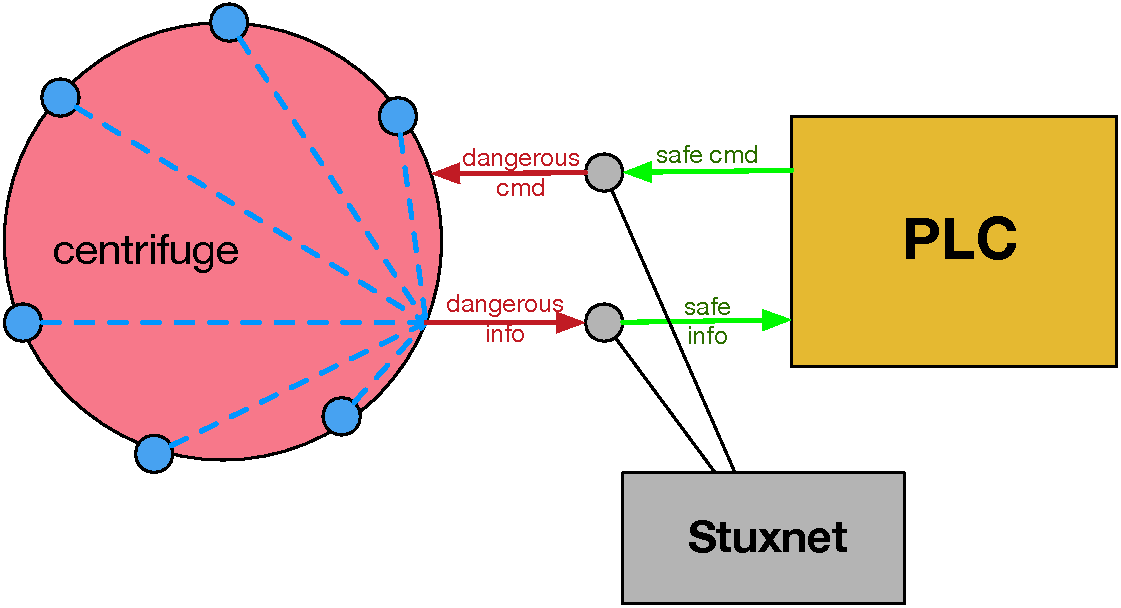
\includegraphics[width=.95\textwidth]{mim}
}
\end{columns} 


 
\end{frame}




\section{Conclusions and Future Work} 


\subsection*{Conclusions} 
\begin{frame}{}
\begin{itemize} 
\item Propose a general declarative framework for representing and reasoning about truthfulness 
 of agents from  
\begin{itemize} 
\item observations about the state of the world;  
\item knowledge about the actions of the agents; and
\item normal behavior of agents.
\end{itemize} 
%\item Evaluate the statements made by agents against a set of observations over time.
\item Develop an implementation in ASP. 
%\item Propose notions of  a supporter (denial) of a statement and discuss possible ways for computing 
%minimal supporter (denial). 
\item Present an application of the proposed framework in 
detecting man-in-the-middle attacks targeting computer and cyber-physical systems.  
\end{itemize}
\end{frame} 
 

%
%
%\begin{block}{Conclusions} 
%Preliminary development of an ASP system for reasoning about truthfulness of statements of agents from 
%observations using default reasoning and reasoning about actions and changes. 

\subsection*{Future Work} 

\begin{frame}{} 

Application of the system in real-world domain:  
\begin{enumerate} 
\item reasoning about reputation of agents (can we trust agent $A$?) 
\item diagnostic reasoning about statements by agents (what should be done to confirm/reject a statement by agent $A$?)  
\item integrating with a model of trust (should I trust information $X$ from agent $A$ given that I trust him only 60\% of the time?)    
\end{enumerate} 

\end{frame}

\begin{frame}{} 

 \center{
Thank you for your attention. \\
} 

 \end{frame}


\begin{block}{References} 
\bibliographystyle{plain}
\bibliography{../bibfile,../bib2010}  
\end{block} 

\end{document} 